\chapter{\IfLanguageName{dutch}{Stand van zaken}{State of the art}}%
\label{ch:stand-van-zaken}

% Tip: Begin elk hoofdstuk met een paragraaf inleiding die beschrijft hoe
% dit hoofdstuk past binnen het geheel van de bachelorproef. Geef in het
% bijzonder aan wat de link is met het vorige en volgende hoofdstuk.

% Pas na deze inleidende paragraaf komt de eerste sectiehoofding.

%Dit hoofdstuk bevat je literatuurstudie. De inhoud gaat verder op de inleiding, maar zal het onderwerp van de bachelorproef *diepgaand* uitspitten. De bedoeling is dat de lezer na lezing van dit hoofdstuk helemaal op de hoogte is van de huidige stand van zaken (state-of-the-art) in het onderzoeksdomein. Iemand die niet vertrouwd is met het onderwerp, weet nu voldoende om de rest van het verhaal te kunnen volgen, zonder dat die er nog andere informatie moet over opzoeken \autocite{Pollefliet2011}.

%Je verwijst bij elke bewering die je doet, vakterm die je introduceert, enz.\ naar je bronnen. In \LaTeX{} kan dat met het commando \texttt{$\backslash${textcite\{\}}} of \texttt{$\backslash${autocite\{\}}}. Als argument van het commando geef je de ``sleutel'' van een ``record'' in een bibliografische databank in het Bib\LaTeX{}-formaat (een tekstbestand). Als je expliciet naar de auteur verwijst in de zin, gebruik je \texttt{$\backslash${}textcite\{\}}.
%Soms wil je de auteur niet expliciet vernoemen, dan gebruik je \texttt{$\backslash${}autocite\{\}}. In de volgende paragraaf een voorbeeld van elk.

%\textcite{Knuth1998} schreef een van de standaardwerken over sorteer- en zoekalgoritmen. Experten zijn het erover eens dat cloud computing een interessante opportuniteit vormen, zowel voor gebruikers als voor dienstverleners op vlak van informatietechnologie~\autocite{Creeger2009}.

%\lipsum[7-20]

Met dit onderzoek is het de bedoeling tot een goed voorstel tot oplossing te komen om de installatie van de nodige software voor de oefeningen van het vak Big Data aan HoGent zoveel mogelijk te automatiseren.
Meer concreet worden tijdens deze oefeningen de applicaties Hadoop, Spark en Kafka gebruikt. Momenteel wordt deze software geinstalleerd tijdens de les zelf en dat is verlies van tijd die nuttiger zou zijn voor het gebruik van de applicaties in plaats van voor de installatie ervan. 

Een extra doelstelling is om deze applicaties ook tijdens de examens te laten gebruiken op een centrale installatie van HoGent, uit veiligheid en stabiliteit.

Voor het gebruik van deze applicaties zijn typisch telkens 2 ervan nodig, bijvoorbeeld Hadoop in combinatie met Spark of Spark in combinatie met Kafka. Meer hierover verder in dit hoofdstuk.

Gezien het doel van deze studie, te komen tot een installatie ter ondersteuning van de oefeningen, zal het onderzoek zich vooral focussen op de functionaliteiten die tijdens de les gebruikt worden en op aspecten van belang voor de installatie, niet op de volledige werking van de verschillende softwares.

We zijn vertrokken van het idee dat de beste aanpak het gebruik van containertechnologie is, die typisch toelaat om dergelijke volledig voorgedefinieerde installaties geautomatiseerd uit te voeren.

\section{Containertechnologie}
Container technology is a lightweight, executable unit of software that packs up application code and dependencies such as binary code, libraries, and configuration files for easy deployment across different computing environments \autocite{Solarwinds2023}.

\subsubsection{Container}
Containers are an abstraction at the app layer that packages code and dependencies together. Multiple containers can run on the same machine and share the OS kernel with other containers, each running as isolated processes in user space. Containers take up less space than VMs (container images are typically tens of MBs in size), can handle more applications and require fewer VMs and Operating systems.\autocite{Docker2023a}

Met containertechnologie wordt de basis van het Operating Systeem gedeeld met de verschillende containers in tegenstelling tot Virtual Machines, die kunnen aanzien worden als een voorganger van containers, waar een volledige `virtuele computer` telkens wordt gebruikt, inclusief het Operating Systeem. Hierdoor zijn containers veel kleiner, zowel wat disk space als geheugen betreft.

De meest gebruikte containersoftware's zijn Docker, CRI-O, rktlet, Containerd en runC. Rekening houdende met andere vereisten, o.a. installatie op het VIC, zie verder, hebben we besloten gebruik te maken van Docker.

\subsection{Docker}
Docker is a software platform that allows you to build, test, and deploy applications quickly. Docker packages software into standardized units called containers that have everything the software needs to run including libraries, system tools, code, and runtime. Using Docker, you can quickly deploy and scale applications into any environment and know your code will run. \autocite{AwsAmazon2023}

Een Docker container wordt gestart op basis van een Docker image, dit bevat alle nodige software en configuratie om een oplossing te kunnen draaien, soms zitten er ook al een deel voorgedefinieerde gegevens in. De container starten betekent het starten van de software in de image, typisch een startup script dat deel uitmaakt van de image.

\subsubsection{Image}
A Docker image is a lightweight, standalone, executable package of software that includes everything needed to run an application: code, runtime, system tools, system libraries and settings.\autocite{Docker2023a}

Docker images gebruiken een `parent` image, bijvoorbeeld een basis Linux container image, waaraan dan via commandos in de Dockerfile (een definitie tekst file) software wordt toegevoegd. De nieuwe image die op die manier wordt gemaakt verwijst naar de parent image maar bevat deze niet. Er wordt een `laag` aangemaakt die dan samen met de parent image kan uitgevoerd worden. Samen vormen ze de nieuwe image.
Deze kan op zijn beurt gebruikt worden als parent voor een andere image, die dan al uit 3 image lagen zal bestaan. Dit vormt een besparing op disk space en netwerk communicatie, want de images worden typisch centraal opgeslagen op DockerHub zodat ze door anderen kunnen gebruikt worden.
Merk op dat dit betekent dat de inhoud van deze image layers niet kan gewijzigd worden, anders zou de container met Image A gebaseerd op Image X de inhoud wijzigen van Image B ook gebaseerd op Image X. Daarom introduceert Docker het concept van een volume. Dit is een opslagplaats waarvan de container kan gebruik maken, maar een volume maakt deel uit van de omgeving waar de container draait, bestaat dus buiten de container en blijft ook bestaan als de container is gestopt. Bijvoorbeeld voor een database container worden de databases zelf in een volume bewaart anders zou alles verloren gaan eens de container wordt gestopt.

\subsection{Volume}
Volumes are the preferred mechanism for persisting data generated by and used by Docker containers.
The data is kept somewhere on storage attached to the host - often the local filesystem. The volume itself has a lifecycle that's longer than the container's, allowing it to persist until no longer needed. Volumes can be shared between containers. \autocite{Javatpoint2023}

Docker containers are used to run applications in an isolated environment. By default, all the changes inside the container are lost when the container stops. If we want to keep data between runs, Docker volumes and bind mounts can help. \autocite{Frieze2022}

Het is hierbij ook good practice/standaard om per image/container maar 1 applicatie te installeren en draaien. Dat maakt het Docker image telkens gelinkt aan 1 oplossing, de meeste uitgevers van software stellen die ook ter beschikking als image op DockerHub, sommige software wordt door derden toegevoegd.

Dus wat we zeker al nodig hebben voor onze oplossing zijn 3 Docker images, 1 voor elke applicatie: Hadoop, Spark en Kafka. Voor alledrie is er een image beschikbaar op DockerHub, die vormen een goede start waaraan we dan zaken kunnen toevoegen indien nodig.

De volgende stap is het automatiseren van het gecombineerd opstarten van applicaties die samenwerken, bijvoorbeeld Hadoop en Spark. Hiervoor kijken we naar een tool `docker-compose` genaamd.

\subsection{Docker-compose}
Docker Compose is a tool that was developed to help define and share multi-container applications. With Compose, we can create a YAML file to define the services and with a single command, can spin everything up or tear it all down. \autocite{Docker2023}

Met een Docker Compose file definieren de verschillende services die samenwerken. Elke service is gebaseerd op een Docker image, per service kunnen we volumes toevoegen, netwerken opzetten die toelaten aan de verschillende containers om te communiceren, dependencies tussen services (welke eerst moet gestart worden), parameters die bepalen wanneer een container moet herstart worden, enz. 

Met 1 docker compose commando wordt de combinatie van services dan opgestart.

Onze oplossing zal dus bestaan uit meerdere docker-compose files, telkens voor een combinatie van de Big Data applicaties.

Aangezien het de bedoeling is om de oefeningen van de studenten zoveel mogelijk van elkaar gescheiden te houden, o.a. om te vermijden dat slechte code van 1 student de applicaties crasht of overbelast, gaan we op basis van de docker-compose files voor elke student een aparte omgeving creeren. Dit betekent dat elke applicatie/container voor elke student apart wordt opgestart maar het is niet de bedoeling dat dit manueel gebeurt, hiervoor bestaat software die toelaat om het beheer van containers te doen, op een automatische manier op te starten, monitoren, herstarten, afsluiten, enz.
In de praktijk wordt bij Docker(Compose) containers Kubernetes gekozen als container management oplossing. Typisch wordt dit ook gebruikt om containers als `cluster` te beheren.

\subsection{Cluster}
A cluster in docker refers to multiple nodes joined. Containers are scheduled across the various nodes, and networking is configured with overlay networking to look similar to bridge networks to the containers, but across multiple nodes.\autocite{BMitch2019}

**********
At a high level, a computer cluster is a group of two or more computers, or nodes, that run in parallel to achieve a common goal. This allows workloads consisting of a high number of individual, parallelizable tasks to be distributed among the nodes in the cluster.
https://www.capitalone.com/tech/cloud/what-is-a-cluster/
**********

Een cluster van nodes/containers gedraagt zich naar de gebruiker toe als 1 enkel systeem, maar het werk wordt verdeelt over de verschillende nodes. Dit laat toe om extra nodes op te starten bij meer belasting en terug af te sluiten om resources te sparen (Scalability), nodes te herstarten zonder dat de gebruiker er iets van merkt (Stability; Availability).

Merk op dat de bedoeling in ons geval eerder is om meerdere `aparte` systemen op te starten, 1 voor elke gebruiker/student dus we gaan daarop focussen bij Kubernetes, de scalability door clustering is een pluspunt indien nodig zou blijken als de belasting zwaarder wordt kan er voor elke student een cluster met meerdere nodes komen.

\subsection{Kubernetes}
Kubernetes, or K8s for short, is an open-source container-orchestration tool designed by Google. It’s used for bundling and managing clusters of containerized applications — a process known as ‘orchestration’ in the computing world.
Kubernetes handles this changeover automatically and efficiently by restarting, replacing, and killing failed containers that don’t respond to a health check.\autocite{Guthrie2022}

We kijken dus naar een oplossing bestaande uit Docker, Docker Compose en Kubernetes die we nu verder gaan onderzoeken, in hoeverre is dit mogelijk op het VIC van HoGent, voor bepaalde combinaties van de applicaties Hadoop, Spark en Kafka.


\section{Hadoop}
The Apache Hadoop software library is a framework that allows for the distributed processing of large data sets across clusters of computers using simple programming models. It is designed to scale up from single servers to thousands of machines, each offering local computation and storage. Rather than rely on hardware to deliver high-availability, the library itself is designed to detect and handle failures at the application layer, so delivering a highly-available service on top of a cluster of computers, each of which may be prone to failures.\autocite{ASF2022}

\subsection{Hadoop Distributed File System}
The Hadoop Distributed File System (HDFS) is a distributed file system designed to run on commodity hardware. It has many similarities with existing distributed file systems.
However, the differences from other distributed file systems are significant. HDFS is highly fault-tolerant and is designed to be deployed on low-cost hardware. HDFS provides high throughput access to application data and is suitable for applications that have large data sets.\autocite{Borthakur2007a}

\subsection{MapReduce}
MapReduce is a programming model or pattern within the Hadoop framework that is used to access big data stored in the Hadoop File System (HDFS). It is a core component, integral to the functioning of the Hadoop framework.
MapReduce facilitates concurrent processing by splitting petabytes of data into smaller chunks, and processing them in parallel on Hadoop commodity servers. In the end, it aggregates all the data from multiple servers to return a consolidated output back to the application.\autocite{Talend2023}
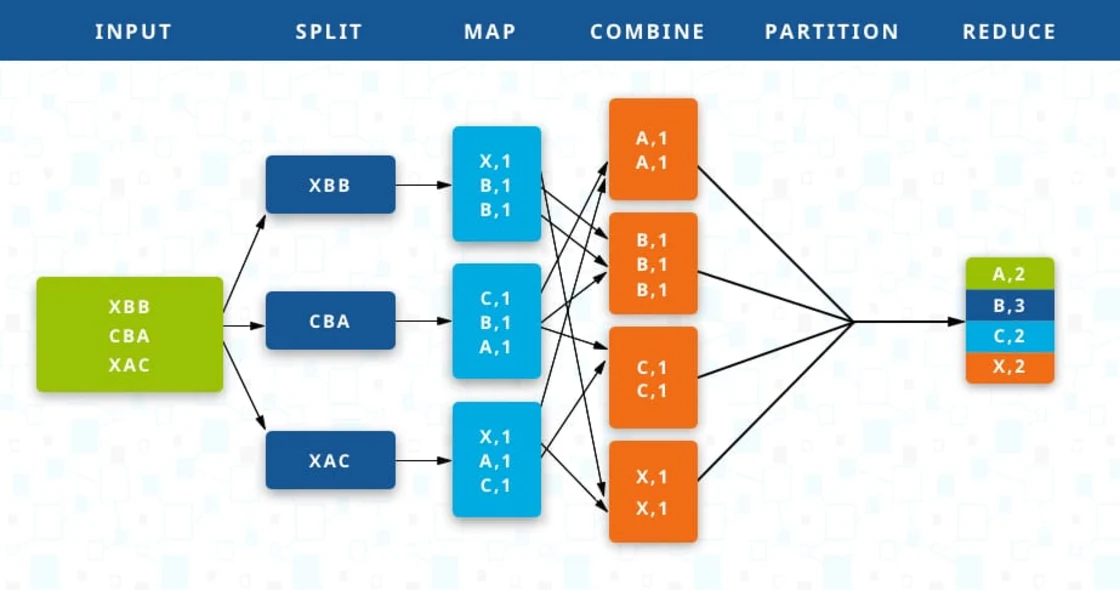
\includegraphics{mapreduce.png}

Hadoop wordt alleenstaand gebruikt tijdens de oefeningen Big Data. 


\section{Spark}
Apache Spark is an open-source, distributed processing system used for big data workloads. It utilizes in-memory caching, and optimized query execution for fast analytic queries against data of any size.
Spark was designed for fast, interactive computation that runs in memory, enabling machine learning to run quickly. The algorithms include the ability to do classification, regression, clustering, collaborative filtering, and pattern mining.\autocite{AwsAmazon2023a}

\subsection{Spark Core}
Spark Core is the underlying general execution engine for the Spark platform that all other functionality is built on top of. It provides in-memory computing capabilities to deliver speed, a generalized execution model to support a wide variety of applications, and Java, Scala, and Python APIs for ease of development.\autocite{databricks2023}

\subsection{Spark RDD}
Resilient Distributed Dataset (RDD) is the fundamental data structure of Spark. They are immutable Distributed collections of objects of any type. As the name suggests is a Resilient (Fault-tolerant) records of data that resides on multiple nodes.
\subsection{Spark SQL}
Many data scientists, analysts, and general business intelligence users rely on interactive SQL queries for exploring data. Spark SQL is a Spark module for structured data processing. It provides a programming abstraction called DataFrames and can also act as distributed SQL query engine. It enables unmodified Hadoop Hive queries to run up to 100x faster on existing deployments and data. It also provides powerful integration with the rest of the Spark ecosystem (e.g., integrating SQL query processing with machine learning).\autocite{databricks2023}

\subsection{Spark MLlib}
Machine learning has quickly emerged as a critical piece in mining Big Data for actionable insights. Built on top of Spark, MLlib is a scalable machine learning library that delivers both high-quality algorithms (e.g., multiple iterations to increase accuracy) and blazing speed (up to 100x faster than MapReduce). The library is usable in Java, Scala, and Python as part of Spark applications, so that you can include it in complete workflows.

\subsection{Spark GraphX}
Apache Spark's API for graphs and graph-parallel computation.
GraphX is a graph computation engine built on top of Spark that enables users to interactively build, transform and reason about graph structured data at scale. It comes complete with a library of common algorithms.\autocite{databricks2023}

\subsection{Spark Streaming}
Many applications need the ability to process and analyze not only batch data, but also streams of new data in real-time. Running on top of Spark, Spark Streaming enables powerful interactive and analytical applications across both streaming and historical data, while inheriting Spark’s ease of use and fault tolerance characteristics. It readily integrates with a wide variety of popular data sources, including HDFS, Flume, Kafka, and Twitter.\autocite{databricks2023}




\section{Kafka}
Apache Kafka is an open-source distributed event streaming platform used by thousands of companies for high-performance data pipelines, streaming analytics, data integration, and mission-critical applications.\autocite{ASF2022b}

Apache Kafka is a distributed data store optimized for ingesting and processing streaming data in real-time. Streaming data is data that is continuously generated by thousands of data sources, which typically send the data records in simultaneously. A streaming platform needs to handle this constant influx of data, and process the data sequentially and incrementally.
\autocite{AwsAmazon2023b}

\subsection{Broker}
A Kafka broker receives messages from producers and stores them on disk keyed by unique offset. A Kafka broker allows consumers to fetch messages by topic, partition and offset. Kafka brokers can create a Kafka cluster by sharing information between each other directly or indirectly using Zookeeper.\autocite{GitBook2023}

\subsection{Topic}
What are Apache Kafka Topics? Apache Kafka has a dedicated and fundamental unit for Event or Message organization, called Topics. In other words, Kafka Topics are Virtual Groups or Logs that hold messages and events in a logical order, allowing users to send and receive data between Kafka Servers with ease.\autocite{Ishwarya2022}

\subsection{Partitions}
What Is a Kafka Partition? In Apache Kafka, partitions are the main method of concurrency for topics. A topic, a dedicated location for events or messages, will be broken into multiple partitions among one or more Kafka brokers\autocite{Carder2022}

\subsection{Offset}
The consumer offset is a way of tracking the sequential order in which messages are received by Kafka topics. Keeping track of the offset, or position, is important for nearly all Kafka use cases and can be an absolute necessity in certain instances, such as financial services.\autocite{Dattell2023}


\section{Zookeeper}
\begin{Zookeeper}
    ZooKeeper is a centralized service for maintaining configuration information, naming, providing distributed synchronization, and providing group services. All of these kinds of services are used in some form or another by distributed applications. Each time they are implemented there is a lot of work that goes into fixing the bugs and race conditions that are inevitable. Because of the difficulty of implementing these kinds of services, applications initially usually skimp on them, which make them brittle in the presence of change and difficult to manage. Even when done correctly, different implementations of these services lead to management complexity when the applications are deployed.\autocite{ASF2023}
    
    What is ZooKeeper in Apache Kafka?
    Zookeeper is used for metadata management in the Kafka world. For example: Zookeeper keeps track of which brokers are part of the Kafka cluster. Zookeeper is used by Kafka brokers to determine which broker is the leader of a given partition and topic and perform leader elections. \autocite{Conduktor2023}
\end{Zookeeper}


Hadoop, Spark en Kafka worden al samen gebruikt volgens \textcite{Holmes2012}:
'In this situation, you'd use Kafka to both land data on Hadoop and provide a feed into a real-time data-streaming system such as Storm or Spark Streaming, which you could then use to perform near-real-time computations.' en \textcite{Leang2019}:
'one of the more significant findings to emerge from this study is that the integration of the Hadoop system especially Apache Kafka and Apache Spark enhances the performance and accuracy of data storing, processing, and securing in the manufacturing environment.'

Er is informatie te vinden over het gebruik van Docker om verschillende combinaties van 2 van de 3 frameworks te installeren maar niks over alle 3 samen, zeker niet met de requirements die wij willen onderzoeken. 

Zoals in meeste momenten word hadoop gebruikt als big data opslag plaats en het verwerkend van big data, spark als real-time data-streaming systeem en kafka als manier om data heen en weer te sturen en hier worden dan combinatie gemaakt met 2 van de 3 voor de gebuiker zijn behoeften. En zoals het ook in de cursus word gebruikt zijn het een combinatie van 2 van de 3.



\section{Virtual IT Company(VIC)}
VIC is een ``bedrijf'' in Hogent dat virtuele machines voorziet voor studenten, zodat bepaalde oplossingen niet op een eigen computer moet draaien, en op aanvraag, er wordt een soort van contract afgesproken met machine specs en lifespan, maken ze de virtuele machine(s).

aan waardoor dit ook zal gebruikt worden voor als doel van dit onderzoek.




\subsection{Hypervisor}
A hypervisor, also known as a virtual machine monitor or VMM, is software that creates and runs virtual machines (VMs). A hypervisor allows one host computer to support multiple guest VMs by virtually sharing its resources, such as memory and processing.\autocite{VMware2023a}


\subsection{VMWare ESXi}
Discover a robust, bare-metal hypervisor that installs directly onto your physical server. With direct access to and control of underlying resources, VMware ESXi effectively partitions hardware to consolidate applications and cut costs. It’s the industry leader for efficient architecture, setting the standard for reliability, performance, and support.\autocite{VMware2023}

\subsection{vCenter}
vCenter Server is the centralized management utility for VMware, and is used to manage virtual machines, multiple ESXi hosts, and all dependent components from a single centralized location. VMware vMotion and svMotion require the use of vCenter and ESXi hosts.\autocite{Abbas2023}

